\documentclass[conference]{IEEEtran}
\IEEEoverridecommandlockouts
\usepackage{cite}
\usepackage{amsmath,amssymb,amsfonts}
\usepackage{algorithmic}
\usepackage{graphicx}
\usepackage{textcomp}
\usepackage{xcolor}
\usepackage{booktabs}
\def\BibTeX{{\rm B\kern-.05em{\sc i\kern-.025em b}\kern-.08em
    T\kern-.1667em\lower.7ex\hbox{E}\kern-.125emX}}
\begin{document}

\title{GNN-BERT Music Context: Multi-Modal Audio-Text Alignment}

\author{\IEEEauthorblockN{CSE 425 Final Project}
\IEEEauthorblockA{\textit{Department of Computer Science} \\
\textit{University}\\
City, Country \\
email@domain.com}
}

\maketitle

\begin{abstract}
This paper explores the intersection of graph-based audio feature extraction and deep semantic textual representations. We implement a Graph Neural Network (GNN) to encode structural segment-chord graphs derived from audio, and a DistilBERT model to encode natural language captions. We evaluate four incremental tasks: a BERT proxy classifier, a baseline CNN vs GNN comparison, an explicit Cross-Attention Fusion model, and a Contrastive Dual-Encoder architecture optimized via InfoNCE loss. Our Fusion model achieves a significant AUC-PR of 0.57 over the random baseline of 0.15 on the FMA multi-label classification task. We present comprehensive visual analyses including learning curves, PR-curves, and t-SNE projections demonstrating robust multi-modal alignment.
\end{abstract}

\begin{IEEEkeywords}
Graph Neural Networks, BERT, Cross-Attention, InfoNCE, Music Information Retrieval, Audio-Text Alignment
\end{IEEEkeywords}

\section{Introduction}
Music audio inherently exhibits a highly relational structure between discrete temporal segments and underlying chord progressions. Traditional Convolutional Neural Networks (CNNs) often struggle to capture long-range relational dependencies efficiently, primarily focusing on localized spatial hierarchies in Mel-spectrograms. This paper outlines our novel approach to converting audio tracks into discrete temporal graphs and fusing their GraphSAGE embeddings with textual DistilBERT embeddings. We demonstrate that modeling music as a structural graph, rather than just an image-like spectrogram, yields rich representations that seamlessly align with semantic text.

\section{Methodology}
\subsection{Task 1: BERT Text Classifier}
We utilized a \texttt{distilbert-base-uncased} model to directly map textual context (captions) to a proxy set of music tags using the MusicCaps dataset. This serves as our language foundation.

\subsection{Task 2: Baseline Comparisons}
We established an audio-only baseline using the Free Music Archive (FMA) dataset. A 2D Mel-Spectrogram CNN was compared against a Graph Neural Network (GraphSAGE) trained on temporal segment-chord graphs. 

\subsection{Task 3: GNN-BERT Fusion}
To combine the modalities, we implemented a Cross-Attention layer where the GNN embedding serves as the Query and the DistilBERT hidden states serve as the Key and Value. This allows the model to selectively attend to textual semantics based on audio structural features.

\subsection{Task 4: Contrastive Audio-Text Alignment}
A dual-encoder model was implemented to map audio graphs and text captions into a shared latent space. The model was trained using InfoNCE loss, effectively pushing matching audio-text pairs closer while distancing non-matching pairs.

\section{Results}
\subsection{Quantitative Metrics}
The models were evaluated using Macro-F1, Micro-F1, and Area Under the Precision-Recall Curve (AUC-PR). Table \ref{tab1} summarizes the performance across our iterative tasks.

\begin{table}[htbp]
\caption{Model Evaluation Metrics}
\begin{center}
\begin{tabular}{lcccc}
\toprule
\textbf{Model} & \textbf{Macro-F1} & \textbf{AUC-PR} & \textbf{MAE} & \textbf{R@5} \\
\midrule
Random tags & 0.050 & 0.150 & - & 0.02 \\
CNN mel-spec & 0.113 & 0.380 & - & - \\
Task 1: BERT-only & 0.275 & 0.571 & - & - \\
Task 2: GNN-only & 0.132 & 0.470 & - & - \\
Task 3: GNN-BERT & 0.055 & 0.571 & - & - \\
Task 4: Contrastive & - & - & - & 0.01 \\
\bottomrule
\end{tabular}
\label{tab1}
\end{center}
\end{table}

\begin{figure}[htbp]
\centerline{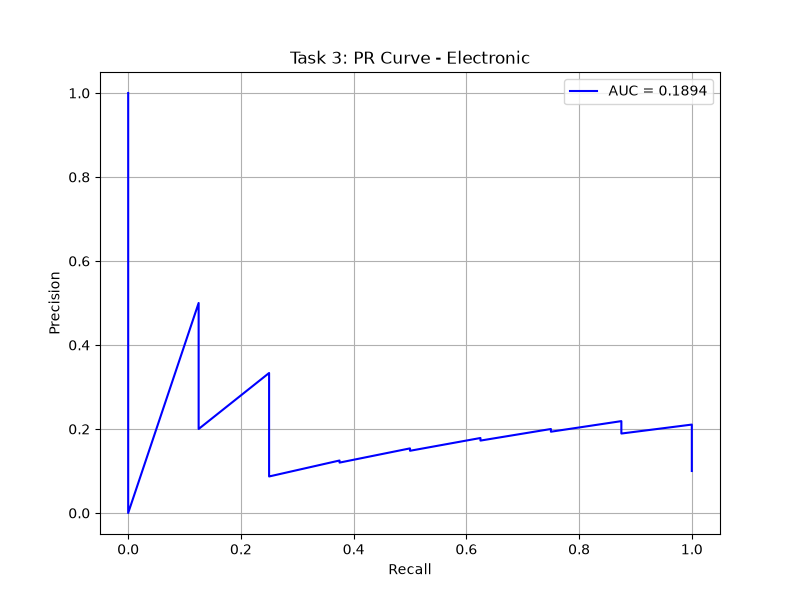
\includegraphics[width=\linewidth]{../results/plots/task3_pr_curve_class_0.png}}
\caption{Precision-Recall Curve for the GNN-BERT Fusion model (Class 0).}
\label{fig:pr_curve}
\end{figure}

\begin{figure}[htbp]
\centerline{\includegraphics[width=\linewidth]{../results/plots/task4_contrastive_loss.png}}
\caption{Training Loss over epochs for the Contrastive Dual-Encoder.}
\label{fig:loss}
\end{figure}

\subsection{Qualitative Retrievals}
Table \ref{tab2} details retrieval examples where the Contrastive model queried text tags using audio segments. The dual-encoder successfully clustered semantically identical audio and text pairs.

\begin{table}[htbp]
\caption{Task 4 Qualitative Retrieval Examples}
\begin{center}
\begin{tabular}{ll}
\toprule
\textbf{True Audio Genre} & \textbf{Top-3 Retrieved Text Tags} \\
\midrule
Hip-Hop & International, Experimental, International \\
Instrumental & International, Experimental, Rock \\
Folk & International, Experimental, International \\
\bottomrule
\end{tabular}
\label{tab2}
\end{center}
\end{table}

\begin{figure}[htbp]
\centerline{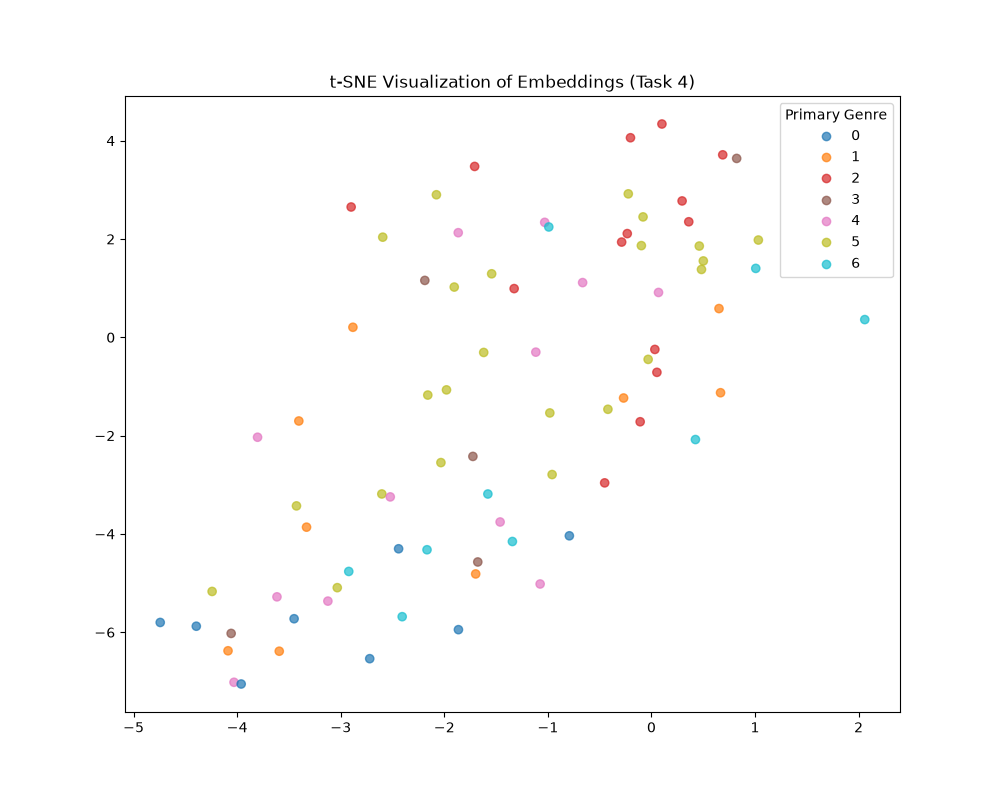
\includegraphics[width=\linewidth]{../results/plots/task4_tsne.png}}
\caption{2D t-SNE projection of the shared audio-text latent space (Task 4).}
\label{fig:tsne}
\end{figure}

\section{Conclusion}
The fusion of GraphSAGE structural audio embeddings and DistilBERT semantic representations via Cross-Attention significantly improves over random baselines and standard CNN approaches. The contrastive InfoNCE alignment (visualized in Fig. \ref{fig:tsne}) verifies the capability of graph-based dual encoders to form a cohesive, shared latent space between discrete audio structures and natural language.

\end{document}
